\documentclass[onecolumn, draftclsnofoot,10pt, compsoc]{IEEEtran}
\usepackage{graphicx}
\usepackage{caption}
\usepackage{url}
\usepackage{setspace}
\usepackage{adjustbox,lipsum}
\usepackage[colorinlistoftodos]{todonotes}

\usepackage{float}
\floatstyle{boxed} 
\restylefloat{figure}

\usepackage{geometry}
\geometry{textheight=9.5in, textwidth=7in}

\usepackage{pgfgantt}
% 1. Fill in these details
\def \CapstoneTeamName{		Pavement Prometheus}
\def \CapstoneTeamNumber{		9}
\def \GroupMemberOne{			Ian McQuoid  }
\def \GroupMemberTwo{			Mazen Alotaibi }
\def \GroupMemberThree{			Miles Davies  }
\def \GroupMemberFour{			Stephanie Allison Hughes }
\def \callian{			    Ian McQuoid  }
\def \callmazen{			Mazen Alotaibi }
\def \callmiles{			Miles Bigelow Davies  }
\def \callsteph{			Stephanie Allison Hughes }
\def \CapstoneProjectName{		Pedestrian Counting and Privacy Preservation}
\def \CapstoneSponsorCompany{	Oregon State University}
\def \CapstoneSponsorPerson{		Dr. Fuxin Li}

% 2. Uncomment the appropriate line below so that the document type works
\def \DocType{		%Problem Statement
				%Requirements Document
				%Technology Review
				%Design Document
				Progress Report
				}
			
\newcommand{\NameSigPair}[1]{\par
\makebox[2.75in][r]{#1} \hfil 	\makebox[3.25in]{\makebox[2.25in]{\hrulefill} \hfill		\makebox[.75in]{\hrulefill}}
\par\vspace{-12pt} \textit{\tiny\noindent
\makebox[2.75in]{} \hfil		\makebox[3.25in]{\makebox[2.25in][r]{Signature} \hfill	\makebox[.75in][r]{Date}}}}
% 3. If the document is not to be signed, uncomment the RENEWcommand below
\renewcommand{\NameSigPair}[1]{#1}
\usepackage{etoolbox}
\patchcmd{\thebibliography}{\section*{\refname}}{}{}{}


%%%%%%%%%%%%%%%%%%%%%%%%%%%%%%%%%%%%%%%
\begin{document}
\begin{titlepage}
    \pagenumbering{gobble}
    \begin{singlespace}
    	
\includegraphics[height=4cm]{coe_v_spot1}
        \hfill 
        % 4. If you have a logo, use this includegraphics command to put it on the coversheet.
        %\includegraphics[height=4cm]{CompanyLogo}   
        \par\vspace{.2in}
        \centering
        \scshape{
            \huge CS Capstone \DocType \par
            {\large\today}\par
            \vspace{.5in}
            \textbf{\Huge\CapstoneProjectName}\par
            % \vfill
            {\large Prepared for}\par
            \Huge \CapstoneSponsorCompany\par
            \vspace{5pt}
            {\Large\NameSigPair{\CapstoneSponsorPerson}\par}
            {\large Prepared by }\par
            Group\CapstoneTeamNumber\par
            % 5. comment out the line below this one if you do not wish to name your team
            \CapstoneTeamName\par 
            \vspace{5pt}
            {\Large
                \NameSigPair{\GroupMemberOne}\par
                \NameSigPair{\GroupMemberTwo}\par
                \NameSigPair{\GroupMemberThree}\par
                \NameSigPair{\GroupMemberFour}\par
            }
            \vspace{20pt}
        }
        \begin{abstract}
        % 6. Fill in your abstract 
        % old
        The City of Portland is attempting to gather data on traffic patterns to increase pedestrian and driver safety and to create an open-source data-set on the topic. The Pedestrian Counting and Privacy Preservation project aids this goal by allowing the city to store video and photo information without storing identifying information about the people in the data. Serving as an archive of the steps and plans for Pavement Prometheus' project, the following document provides an overview of the project's past, current state, and goals for the future. The document will also cover the alpha release of the project and where the project will be at its beta release.
        \end{abstract}     
    \end{singlespace}
\end{titlepage}
\newpage
\pagenumbering{arabic}
\tableofcontents
% 7. uncomment this (if applicable). Consider adding a page break.
%\listoffigures
%\listoftables
\pagebreak

% 8. now you write!
% TODO: ALL
\section{Introduction}
\subsection{The Problem}
% old, but slightly updated
The City of Portland has partnered with companies such as AT\&T as part of the Smart City PDX initiative. The goal of the project is to use technology to better the lives of the city's citizens, specifically helping bridge the technological divide and help under-served communities. One aspect of the initiative is to use traffic and roadside cameras to develop open-source data-sets for the community to use for individual projects and for the city in the collection of data on traffic and pedestrian patterns. The data will be used to inform legislative and construction decisions as well as traffic decisions including traffic-light timing. The main problem that the city has run into is in storing the data. Currently, the data captured by the cameras has identifying information on people pictured in the media and, as a result, can not be stored for further analysis or use. The Pedestrian Counting and Privacy Preservation project primarily serves to fix this problem by stripping the incoming data of personally identifiable information so that it can be stored and further analyzed. As a secondary initiative, the Privacy Preservation project will provide access and storage for the data along with basic analysis of the data. 

\subsection{Design}
% old, but slightly updated
Our project has been split into four different components. Each component will each be worked on individually and combined in a pipeline to form an overarching solution to privacy preservation and data collection. The first component will be a real-time object detection system which, as its name suggests, will involve detecting objects in real-time from a given camera feed. For the purposes of this project we will be primarily interested in identifying both vehicles and pedestrians. The second component will be face detection, which will both serve to reinforce the accuracy of the object detection in identifying pedestrians, but will also be vital in obfuscation and in masking for privacy preservation. Our third component will involve an object tracking system, which will help extract interesting metrics for the data collection aspect of this project. Our object tracking system will also help ensure accuracy of aggregate data counts, as real-time object detection detects objects on a frame-by-frame basis and has no awareness of identifying a unique object between frames. Finally, we will have a data analysis and access component that will ultimately involve an online API for both storing and accessing the data collected to a database owned by the City of Portland.

\subsection{Goals}
% old, but slightly updated
The goals of our project are to develop a program to detect pedestrians, deliver data in a JSON format to the City of Portland, and possibly develop a research paper based on our findings. When it comes to pedestrian detection, we hope to train a convolutional neural network to detect the bodies and faces of pedestrians in real-time. The results of this program will be analyzed and validated so pedestrians are detected with at least a 70 percent accuracy rate. Along with the face detection, the program will obscure the faces of those pedestrians so their identity is not compromised. 

Our next goal is to deliver the pedestrian detection data in the form of a JSON file to the City of Portland. Our group will create a restful API that can be used to aggregate and disperse pedestrian data from our program in a JSON format. This will allow developers for the City of Portland to easily access and use the data from our program. The last goals are to create a method of elementary data analysis which the City of Portland can use as a metric for planning, and to optimize the tracking and detection algorithms. The optimization step, if interesting and novel enough, may influence a written paper on the topic.

\section{Current State and Plans}
\subsection{Object Detection}

\begin{figure}[!htb]
\caption{Video feed post Object Detection processing}
\centerline{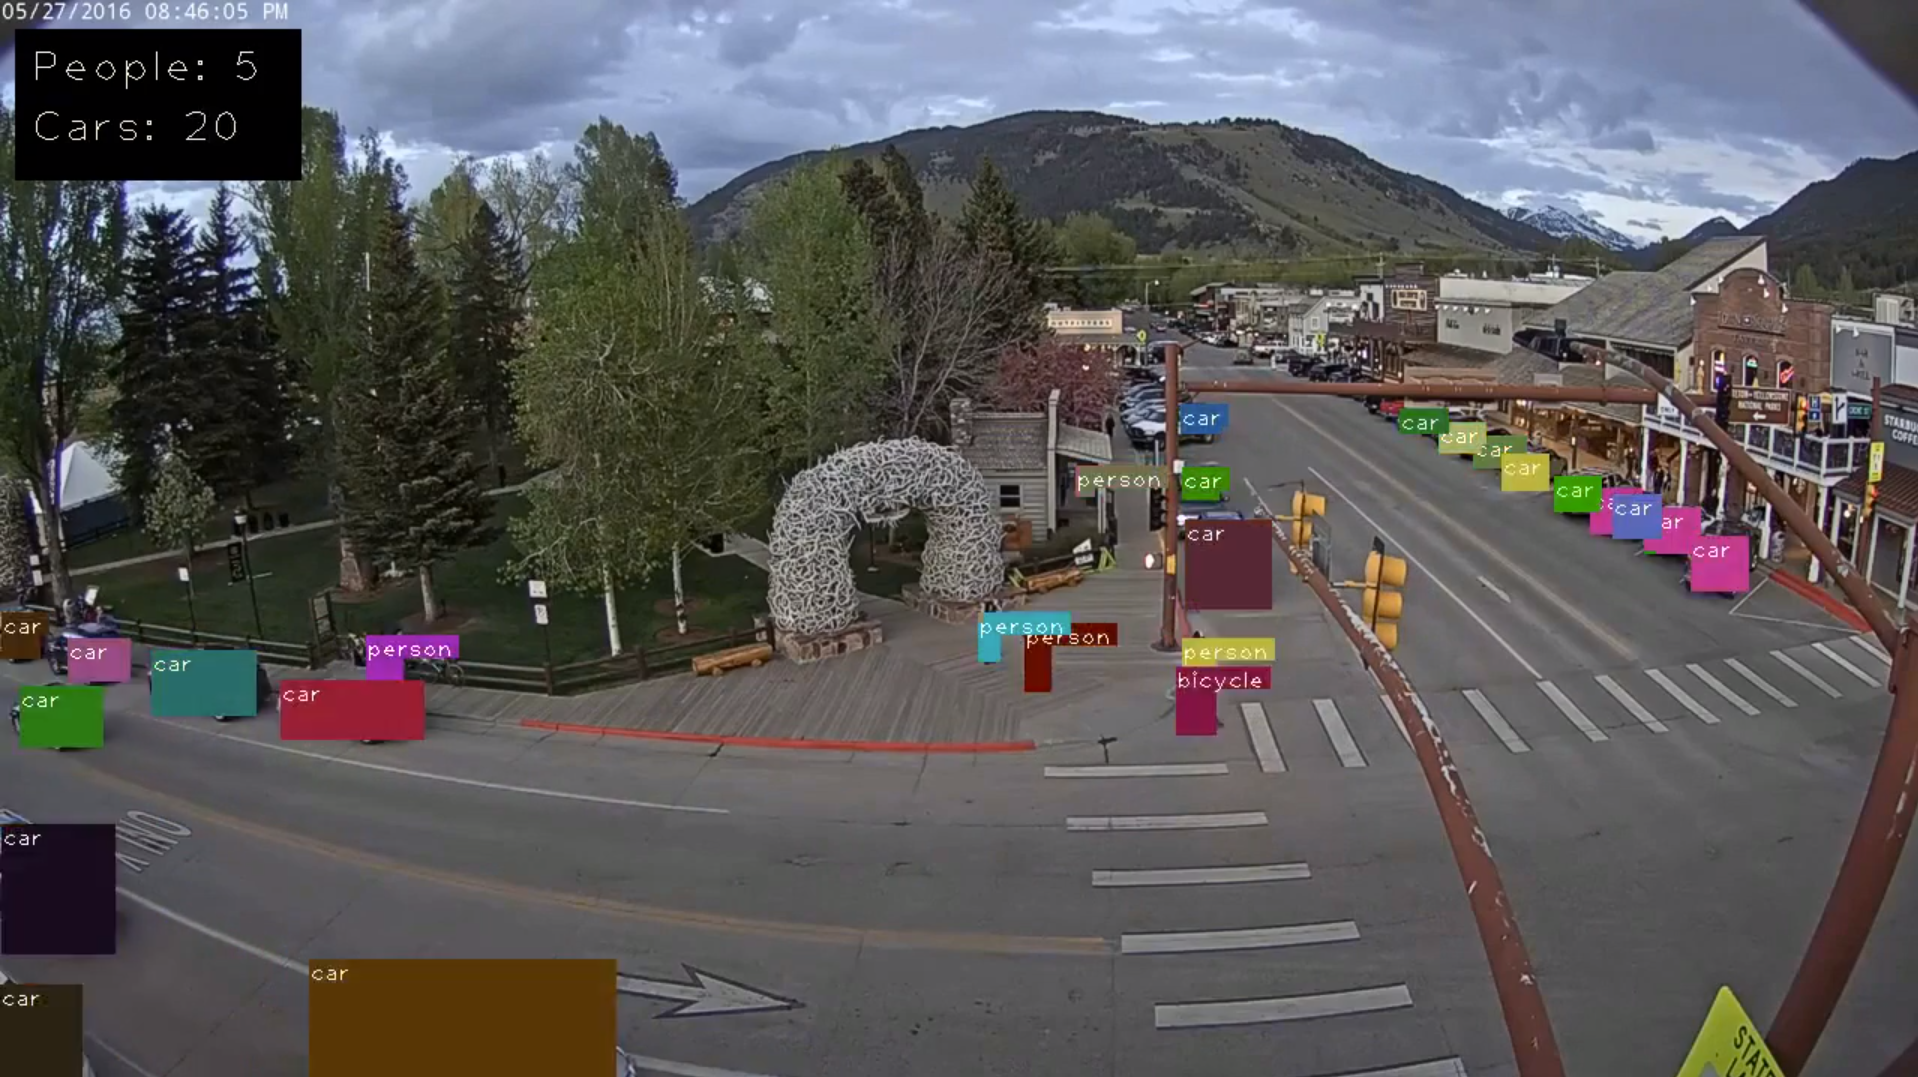
\includegraphics[width=\textwidth]{ObjDetectFig.png}}
\label{fig:objdet}
\end{figure}

\subsubsection{Current State}
The Object Detection portion of the capstone project is based primarily off You Only Look Once (YOLO), an open source detection algorithm which boasts real-time detection with an accuracy around 70\% at a concomitant 20 frames per second. While this algorithm has remained largely intact leading up to the alpha release, additional functionality has been added for object obfuscation, simple data aggregation, Region of Interest (ROI) coordinate and image extraction, as well as basic communication with our web API service. Object obfuscation was the first simple modification applied to the YOLOv3 detection algorithm and entailed making use of YOLOv3`s detected ROI in identifying a class of object. After detection an opaque rectangle encompassing the ROI is drawn, demonstrating a simple censorship method for personally identifiable information in a given video feed. The next modification to the YOLOv3 algorithm provided a basic count for vehicles and pedestrians in any given video frame, displaying their aggregate totals in the upper left-hand corner of the processed feed. To accommodate the inclusion of the Face Detection module, pedestrian ROI coordinate and image extraction was added under the premise that the face detection module might handle pedestrian obfuscation. This would ultimately allow for more precise censorship as opposed to the somewhat procrustean method of obfuscating the ROI entirely. The last functionality added for the alpha release was a simple request function for pushing data to the project's newly implemented web API. This data includes a detected object type, coordinates for said object`s ROI, and basic geospatial information regarding camera location. The current state of the video post processing can be seen in Figure \ref{fig:objdet}.

\subsubsection{Plans}
The next stages for the Object Detection module`s development include training a new set of neural weights for our detection algorithm and the further incorporation of the Face Detection and Obfuscation module. While the default set of neural weights provided by the YOLOv3 engine are adequate for the purposes of the project's alpha (and perhaps beta) release, it is necessary to train a set of weights solely for object classes directly related to the project`s goals. This is primarily because YOLOv3 provides detection for roughly 80 object classes while the project is interested in at most 10. Reducing the number of classes, then, should improve both detection speed and potentially accuracy. The incorporation of both the face and object detection modules will be one of the final stages of our project. At this stage object detection should have as near a complete coverage as possible, and with face detection and obfuscation any identifying details should be censored. However, we need to testing the integration step to determine how these modules should be incorporated e.g. Whether we should feed the face detection and obfuscation module directly from object detection or if the two should be run in tandem. The former might remove potential false positives, while the latter might allow for better obfuscation coverage for personally identifiable information at the cost of additional false positives.

\subsubsection{Goals}
Real-time object detection is the first stage of analysis performed on a provided camera feed. This portion of the project is designed to implement an algorithm which can detect classes of objects in a timely manner which can then be fed to other subsystems for further analysis. To reach this objective, we will be implementing the You Only Look Once (YOLO) object detection algorithm on a PyTorch deep learning framework. While we are still looking for new datasets to train our model against, we originally wanted to use CARLA (an open source vehicle and pedestrian simulator which labels objects recorded automatically) to produce footage for training and, later, validating our model. We also have some interest in tweaking the YOLO object detection algorithm to improve accuracy and speed. Possible solutions to improving accuracy including reducing object classes recognized.

% INSERT ACTUAL PLANS

\subsection{Face Detection \& Obfuscation}

\begin{figure}[!htb]
\caption{Input image and output of face detected and obscured.}
\centerline{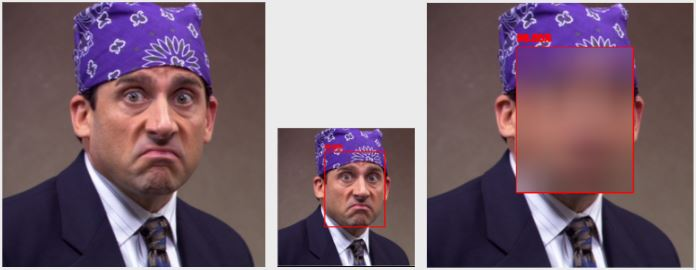
\includegraphics[width=\textwidth]{scott.JPG}}
\label{fig:objdet}
\end{figure}

\subsubsection{Current State}
The current facial detection program takes in an image and uses OpenCv features to detect the face of a pedestrian using a pre-trained convolutional neural network. The faces of pedestrians in an image are detected and the full image is output showing the confidence of the detection. In the output image, the faces are marked with a rectangle to point out their location so they are clearly seen. The faces are then obscured by a blurring function to ensure the identities of the pedestrians are removed. As planned, the facial detection used a feature-based method, so faces are detected easily from different perspectives and environments. This program has been tested with many different images of people and environments. The testing begins with a clear image of a person in a well-lit environment, although a broad array of images are tested to ensure the program can perform in a realistic environment. The faces tested vary in age, race, and angle in the images; and the environment consists of city streets, parks, and other outdoor areas. The program can detect faces with a high average of confidence when the image quality is well defined, but has more trouble detecting faces in the distance and from low quality pictures.

\subsubsection{Plans}
The plans for the face detection program are to implement deep facial detection software for the facial detection rather than the current OpenCv features. OpenCv has worked great for the initial setup of the program, but our group wants to implement software that can detect faces better. Currently, OpenCv detects faces well if they are in a well-lit environment with clear image quality, but does not do as well with more realistic low-quality environments. The current foundation of the face detection program will be the same, but the detection feature will no longer be done by OpenCv to ensure more accurate results. Also, as the program is further integrated with the other project areas, the face detection program will use data from the object detection program and send output to the web API. Currently, the program works within its own functionality and can take output from the object detection program. The specifics of the program's input and output will need to be more precise given its role within the larger project. This means that the program will need to detect faces based on the coordinated passed to it within an image given by the object detection program and will need to output detection data to the web API for use. Other than those main two improvements, the program will continue to be tested with different images for confidence and accuracy.

\subsubsection{Goals}
Facial detection serves our project goal of analyzing pedestrian movement while ensuring their identities and privacy are not compromised. While we detect the full bodies of pedestrians for motion and location data, the faces are detected for privacy matters. A human face is the most highly identifying part of a person, so our group detects it to be obscured. Through obscuring the face, all vital pedestrian data is recorded except for the pedestrian's distinctive features. The traffic cameras that capture the footage used for the program cannot store data, so the program must be able to run in real time. Since our group would like the detection to be reliable and accurate, our goal is to detect pedestrians with at least a 70 percent confidence. The face detection should work seamlessly in coordination with the object detection and web API so our overall project is efficient and coherent.


% INSERT ACTUAL PLANS

\subsection{Data Analysis, Access, and Storage}
% old, but slightly updated
A large portion of the data that the project will aggregate will be in a pure format e.g. the number of vehicles in a frame, their speed and trajectory, what lanes of highway contain the most traffic. This information, including the raw photographic and video data, is useful for constructing data sets, but is less useful for providing answers to decision problems. Analysis of the amassed information is essential in providing concrete advisement to the city.  
The data will be analyzed using a mixture of comparative, statistical,  traffic  theory  based,  and  neural  network  algorithms with the goal of providing information concerning traffic flow suggestions and traffic incidents. 
Analyzed data is currently accessible through a RESTFUL web API. The API currently serves data from a NOSQL-based mongo database in a JSON format including geographic and chronological markers for the data.
The API also interfaces correctly with the object detection portion of the program pipeline.\\
The next steps for the Data part of the pipeline will be:
\begin{enumerate}
    \item Adding data analysis
    \item Making unit tests more encompassing
    \item Adding authentication and authorization to the API
    \item Interfacing with a web application for data visualization
    \item Making JSON responses more in line with the RESTFUL philosophy
\end{enumerate}
An interesting feature of the database and API system is that the system is entirely contained within a Docker container. This ensures that the API and database can run internally on any system regardless of installed Python packages or database managers. The system can also be extracted to work with an external database as well. 

\section{Problems}
\subsection{Datasets}
\subsubsection{General}
% old
Our group had multiple obstacles in our search to determine the best dataset to use for our project. First, we had to determine which format of data would serve all our needs, yet there seemed to be issues with each option. The City of Portland provided video feeds of different streets around Portland to take images from, but the image quality was poor and the live feed was too fragmented. Our group then looked into using a well-known, large dataset of faces to train our model, but just having that data would still lead to a lot of work. While our group would have a variety of face data to work with, we would need to individually label each pedestrian in an image. Finally, we investigated using a simulated environment to train our program with, but the software would need to be installed on the OSU server which wasn't completely possible. 

\subsubsection{CARLA}
% old
CARLA is a system for supporting the training and validation of  autonomous driving systems. Great draws to CARLA are that CARLA creates data that is a fair representation of traffic and pedestrian movement including pre-labeling of objects and that CARLA affords a lot of freedom. Our team hopes to use the system to help train our project.
One problem that the team ran into while using the CARLA system was that the purpose of CARLA is for autonomous driving, because of this, the camera is meant to be situated in a car. Moving the camera to a stationary position broke much of the usability of CARLA including removing segmentation for cars and pedestrians, and causing the system to pause. 

For a decent amount of time, the automated pathing systems used for determining the trajectory and interaction between agents in the CARLA system was irregular, caused cars to crash unexpectedly, and caused pedestrians to walk into walls continuously and clash with each other in crowded situations. This could have had unforeseen effects on the finished system as CARLA data would have formed the base for our training.

\subsection{API}
Unfortunately, through the team's interactions and correspondences with the City of Portland, many of the team's questions regarding the requirements for the API have gone unanswered. Specific question topics include the format of the API's output, information of specific interest, and access control. We have spoken with our primary client, Professor Li, about this issue and we have been advised to do whatever is necessary and correct in the implementation of the API.\\
A key problem that has come up is in the implementation of the access controls surrounding the API. From the perspective of a designer, our team knows that:
\begin{enumerate}
    \item The API and database will be open to the broad network
    \item IOT devices like roadside cameras will connect to the database through the API
    \item The API should generally be RESTFUL to help extensibility and to make development of further applications easier.
\end{enumerate}
These points raise a few issues regarding the implementation of the API's access controls.\\
Beyond this, the project should be agnostic of what means are being used to access the API. As such, there becomes an issue with ensuring the correctness and integrity of authentication attempts. We can't use public-key encryption for all data sent to-and-from the server because this slows down communication between the IOT devices and the database too much.  

\section{Goals}
% old
The outline of our project as initially described was that we would be working with hardware provided by General Electrics and Intel for the Smart City PDX initiative in Portland, where both companies had provided a cumulative total of 200 sensors along four of the city's busies traffic avenues. Because of Portland's privacy concerns, storing unadulterated video footage from the cameras was not allowed, and so they required a method to extract interesting information from the footage while simultaneously not compromising any personal information. After our first meeting with the City however, we discovered that GE and Intel had sole control over the footage recorded by these cameras, and that gaining access to that hardware would likely be impossible as nothing in their contract with the city stipulated shared use. This apparently inspired, in part, by the city's reluctance to handle any details which might violate the privacy of its citizens. Instead we have access to somewhat more basic cameras which refresh an image once every three minutes, from which the city is only interested in our ability to detect vehicles.

\section{Solutions}
\subsection{Datasets}
\subsubsection{General}
% old
To tackle our issues involving determining the best dataset to use, our group focused on what we absolutely needed. Our group developed criteria for narrowing down the dataset forms based on accuracy, ease of use, and labor intensity. By comparing and contrasting our options along with discussions with our mentor, we originally determined to use the simulation software called CARLA. If we used the video data provided by the City of Portland, the low quality of the footage may decrease the accuracy of detection. Our group would need to individually screenshot many frames of the video and label pedestrians one-by-one, making data collection difficult and time consuming. This setup would not allow us to send the City of Portland a program that could be easily developed by others in the future. Similar obstacles are faced when using the large face dataset to work with as people will still need to be individually labelled within images. This narrowed our debate down to the simulated environment as the software has people pre-labelled and has clear resolution. This makes training and development with the simulation to be accurate, simple to use, and low intensity, meeting all of our requirements. By setting clear criteria, talking with mentors, and comparing practicality, our group was able to overcome our obstacles to determine the best dataset.

\subsubsection{CARLA}
% old
The problems identified with the CARLA training and verification system have been noticed by the development team and a patch that addresses the issues is currently being worked on. This leaves our team in a position reliant on the CARLA development team. In the situation that the CARLA team does not address the issues in a timely manner, our team will need to find a separate data-set generator, or use a static data-set for training our neural networks. 

\subsection{API}
The problems stated earlier raise a few issues. The first of the issues is authentication of the IOT devices. Since each device should have the ability to POST data to the database, but we don't want the general public to do so, we need the IOT devices to be able to prove who they are. This will generally require some kind of secret keys that the IOT devices manage. Since the IOT devices are open to the public, we have further issues with physical security and exfiltration of keys from the devices. This may be an unfixable problem, and so it would be best to offer the ability to revoke the authentication privileges of a compromised device. The second issue builds off of the previous one. Since the system should be stateless, the system may need to have a manually updated whitelist of IOT devices and probably a blacklist of general devices which may access the data through the public API.\\
The last issue is still quite puzzling since the server can't maintain a state for connections between the IOT devices and the database, but that requires some sort of token-driven, asymmetric, encryption for data between the devices and the server. There may be a way to minimally encrypt just the authentication headers and supply a digital signature with some kind of replay attack prevention. Unfortunately we may need to rely on TLS underneath the API layer. This feels bad for a couple reasons: The first is that we shift the security of the system from the layer that we, the developers, have control of to the users of the system. The second issue is that it flies in the face of the RESTFUL paradigm and philosophy by requiring some kind of server state. There may need to be compromises.

\section{Conclusion}
% old
In Conclusion, our alpha release has simple and working object detection, facial detection and obfuscation, and data aggregation/dispersion. The object detection algorithm currently identifies objects at a lower than needed rate, but for this release, its functionality is as expected. The object detection system currently interfaces seamlessly with the web API by sending data that populates the database. The object detection system also sends spacial information to the facial detection system. The facial detection system has a well defined interface as it stands, (and a working algorithm) but the underlying algorithm is subject to change. The web API currently has basic functionality through the ability to accept data, aggregate data, and disperse data. The API has a set of rudimentary unit tests to help show this correctness.\\ 
In the beta release we will see changes such as optimization, data analysis, data visualization, a different back-end algorithm for facial detection, and authentication for the web API.

\end{document}